\section{Suffix Tries}

Let us recall the definition of a suffix.

\begin{definition}[Suffix] \index{suffix}
    For any string $S$, $S[i\ldots j]$ is the \textit{\textbf{substring}} starting at position $i$ and ending at position $j$; $S[1\ldots i]$ is the prefix of $S$ ending at $i$; and $S[j\ldots |S|]$ is the \textit{\textbf{suffix}} of $S$ starting at position $j$. A proper substring, prefix, or suffix is a substring, prefix, or suffix that is neither the entire string $S$ nor the empty string.
\end{definition}

Then, we define a trie and a suffix trie as follows.

\begin{definition}[Suffix Trie] \index{trie} \index{suffix trie}
    A \textit{\textbf{trie}} is the smallest tree such that each edge is labeled with a character from the alphabet $\Sigma$, each node has at most one outgoing edge labeled with $c$ for each $c \in \Sigma$, and each node has a key that is the concatenation of the edge labels along the path from the root to that node. A \textit{\textbf{suffix trie}} is a trie where each root-to-leaf path represents a suffix.
\end{definition}

\begin{figure}[htbp]
    \centering
    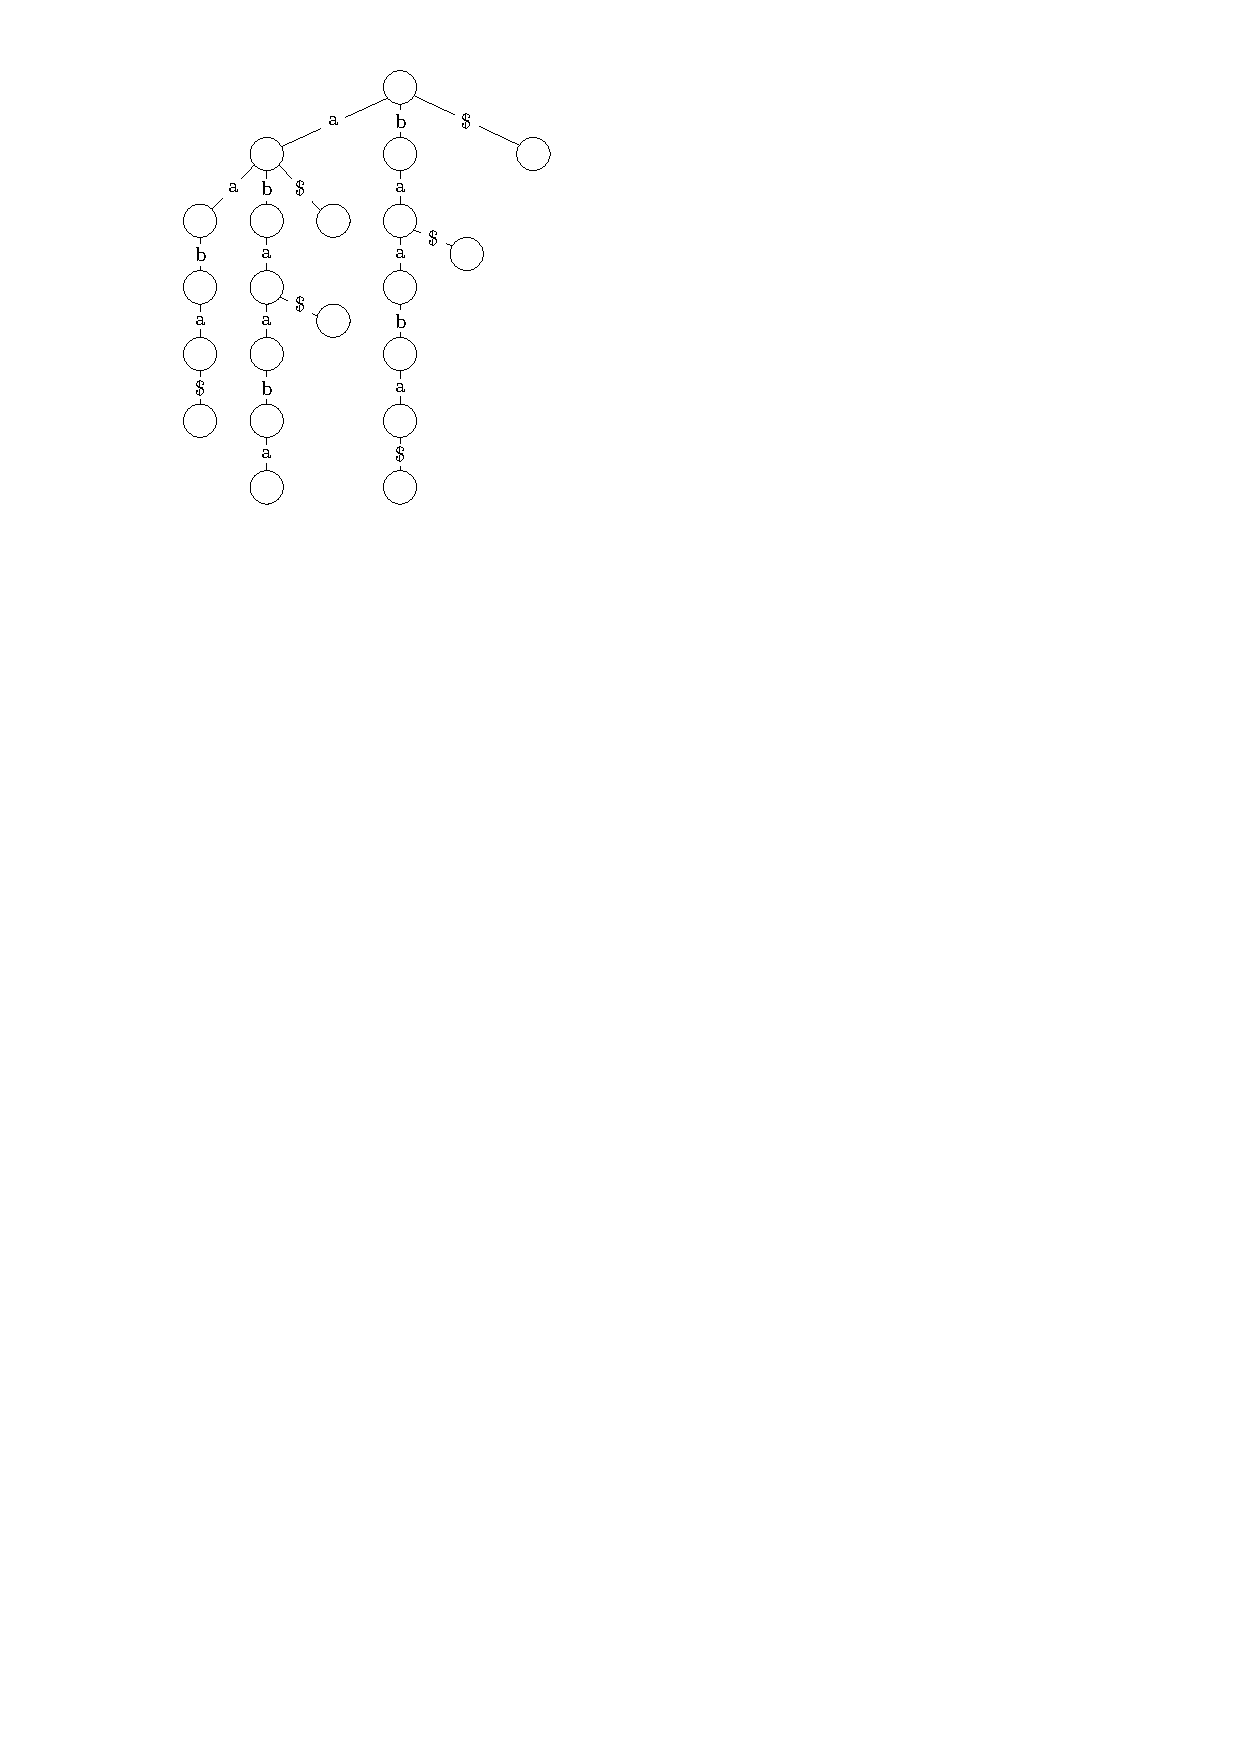
\includegraphics[width=0.45\linewidth]{suffix-tree/suffix-trie.pdf}
    \qquad
    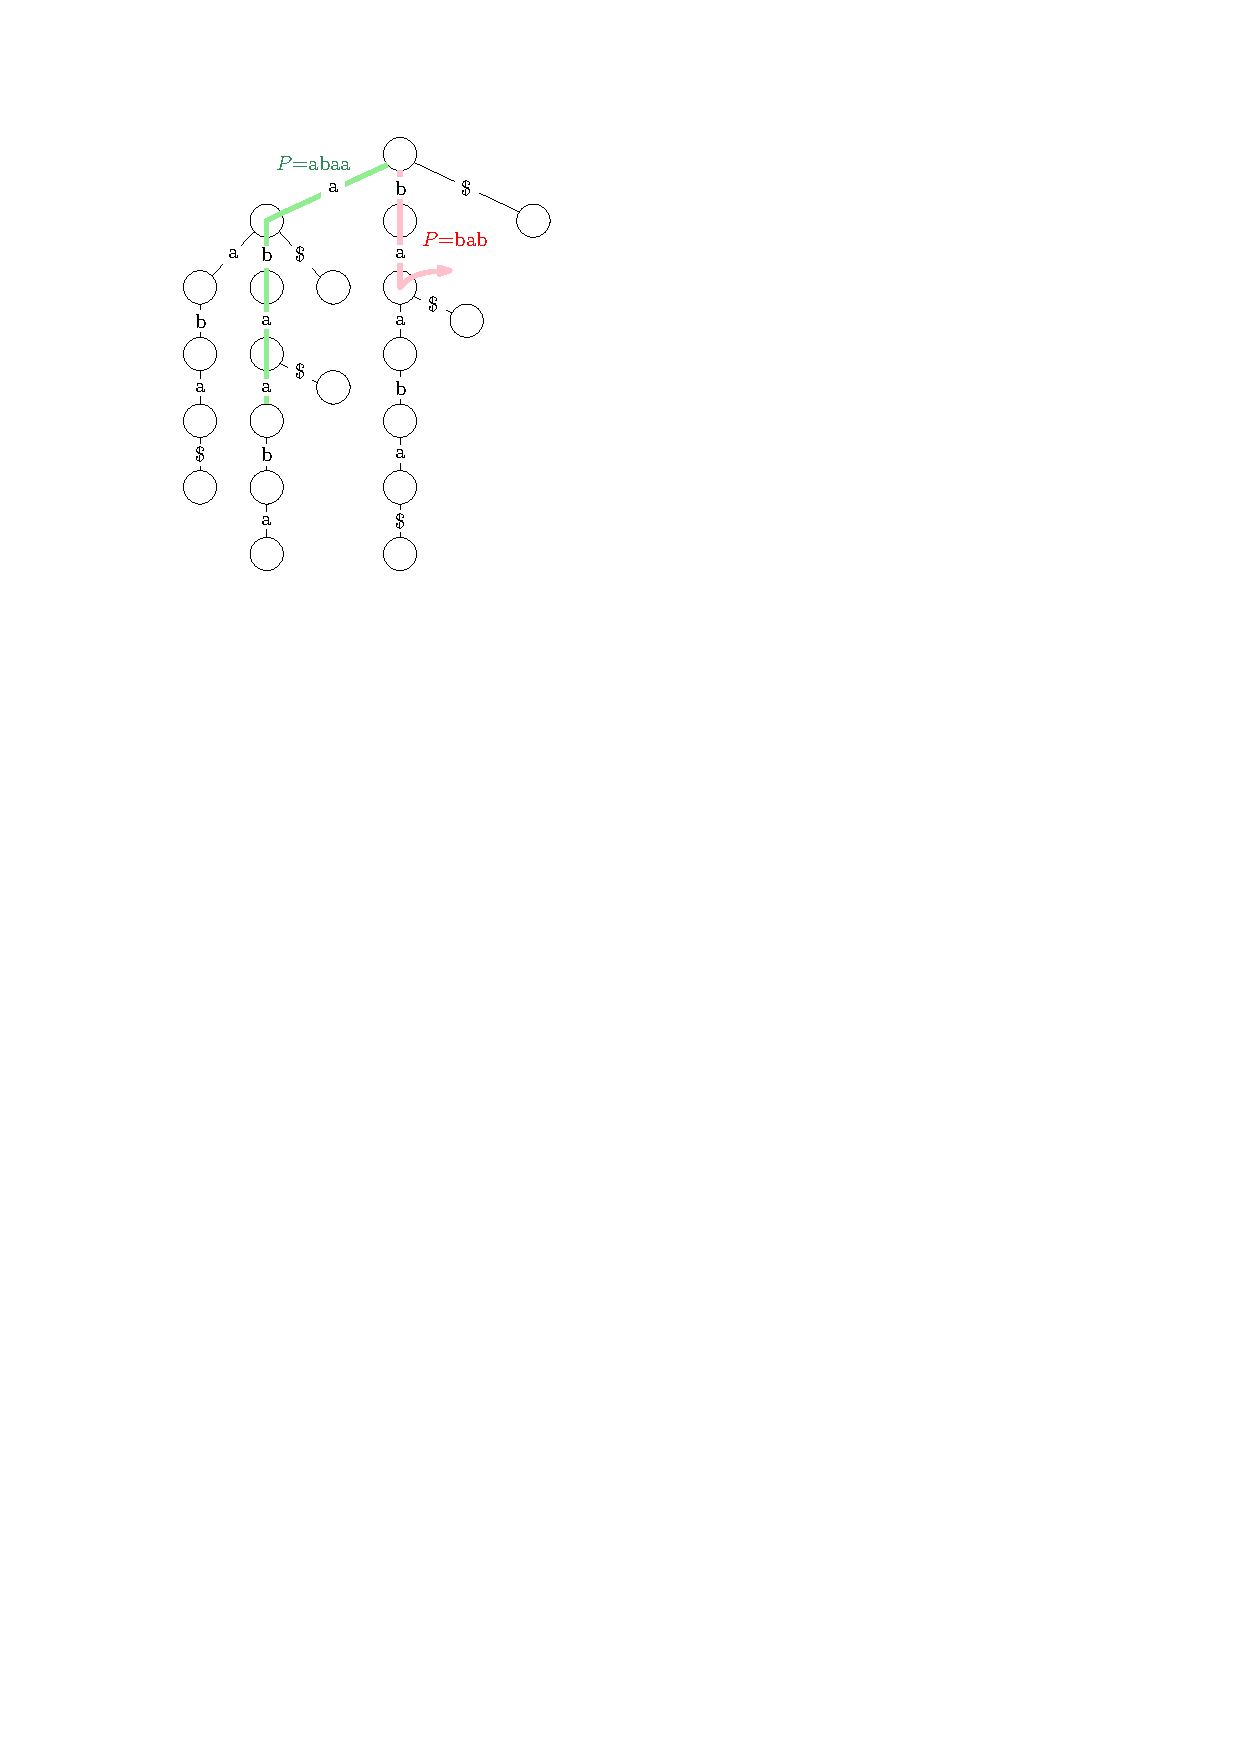
\includegraphics[width=0.45\linewidth]{suffix-tree/suffix-trie-search-path.pdf}
    \caption{Suffix trie for $T = abaaba$. On the right: the search path for $P=abaa$ and $P=bab$. When searching for a pattern that is not in $T$, we ``fall off'' the trie.}
    \label{fig:suffix-trie}
\end{figure}

In a regular tree (e.g. binary search tree), the key is stored at each node. In a trie, the keys are \textit{implicitly} represented by the edge labels along the path. Figure \ref{fig:suffix-trie} shows a suffix trie constructed for $T = abaaba$.

It is important to add the terminator character \texttt{\$} at the end of the string. If we remove the terminator \texttt{\$}, it is not hard to see the result trie may no longer be a valid suffix trie. We assume that \texttt{\$} is \textit{lexicographically smaller than all characters} in $\Sigma$.

\subsection{Search in Suffix Trie}

\newthought{Search for Pattern}: It is easy to search for a pattern $P$ given a suffix trie. We can \textbf{start from the root and follow the edges labeled with the characters} in $P$ until we either finish reading the pattern and find a match, or ``fall off'' the trie, in which case we can return that a match is not found.

\begin{codebox}
    \Procname{$\proc{Search-Trie}(P,T)$}
    \li $\id{cur} = \attrib{T}{\id{root}}$
    \li \For $c$ \textbf{in} $P$ \Do
        \li \If $c \not\in \attrib{\id{cur}}{edges}$ \Then
            \li \Return \const{false}
        \li \Else $\id{cur} = \attrib{\id{cur}}{edges}[c]$
        \End
    \End
    \li \Return $\id{cur} \neq \const{null}$ 
\end{codebox}

Assume that at each node, we maintain a hash table for each outgoing edges. Then, the algorithms runs in expected time $\Theta(|P|)$.

\newthought{Search for Suffix}: Similarly, if we want to see if a given pattern $P$ is a suffix of $T$, we can run the same algorithm and checks if the node at the end of the path has an outgoing edge labeled \texttt{\$}.

\newthought{Search for Number of Occurrences}: If we are interested in the number a pattern $P$ occurs as a substring in $T$, we can run \proc{Search-Trie}. Once we arrive at the end of our search path, we run a \textbf{depth-first search} from the node at the end of the search path and count the number of leaf nodes reachable from that node. Since a trie is a tree, DFS runs in $O(|V|)$ time. In this case, it takes $O(|P|+|T|)$ time to find the number of occurrences of a given pattern.

\textsc{Search for Longest Repeated Substring}: Find the deepest (internal) node with more than one children.

\subsection{Space Complexity of Suffix Trie}

\begin{marginfigure}
    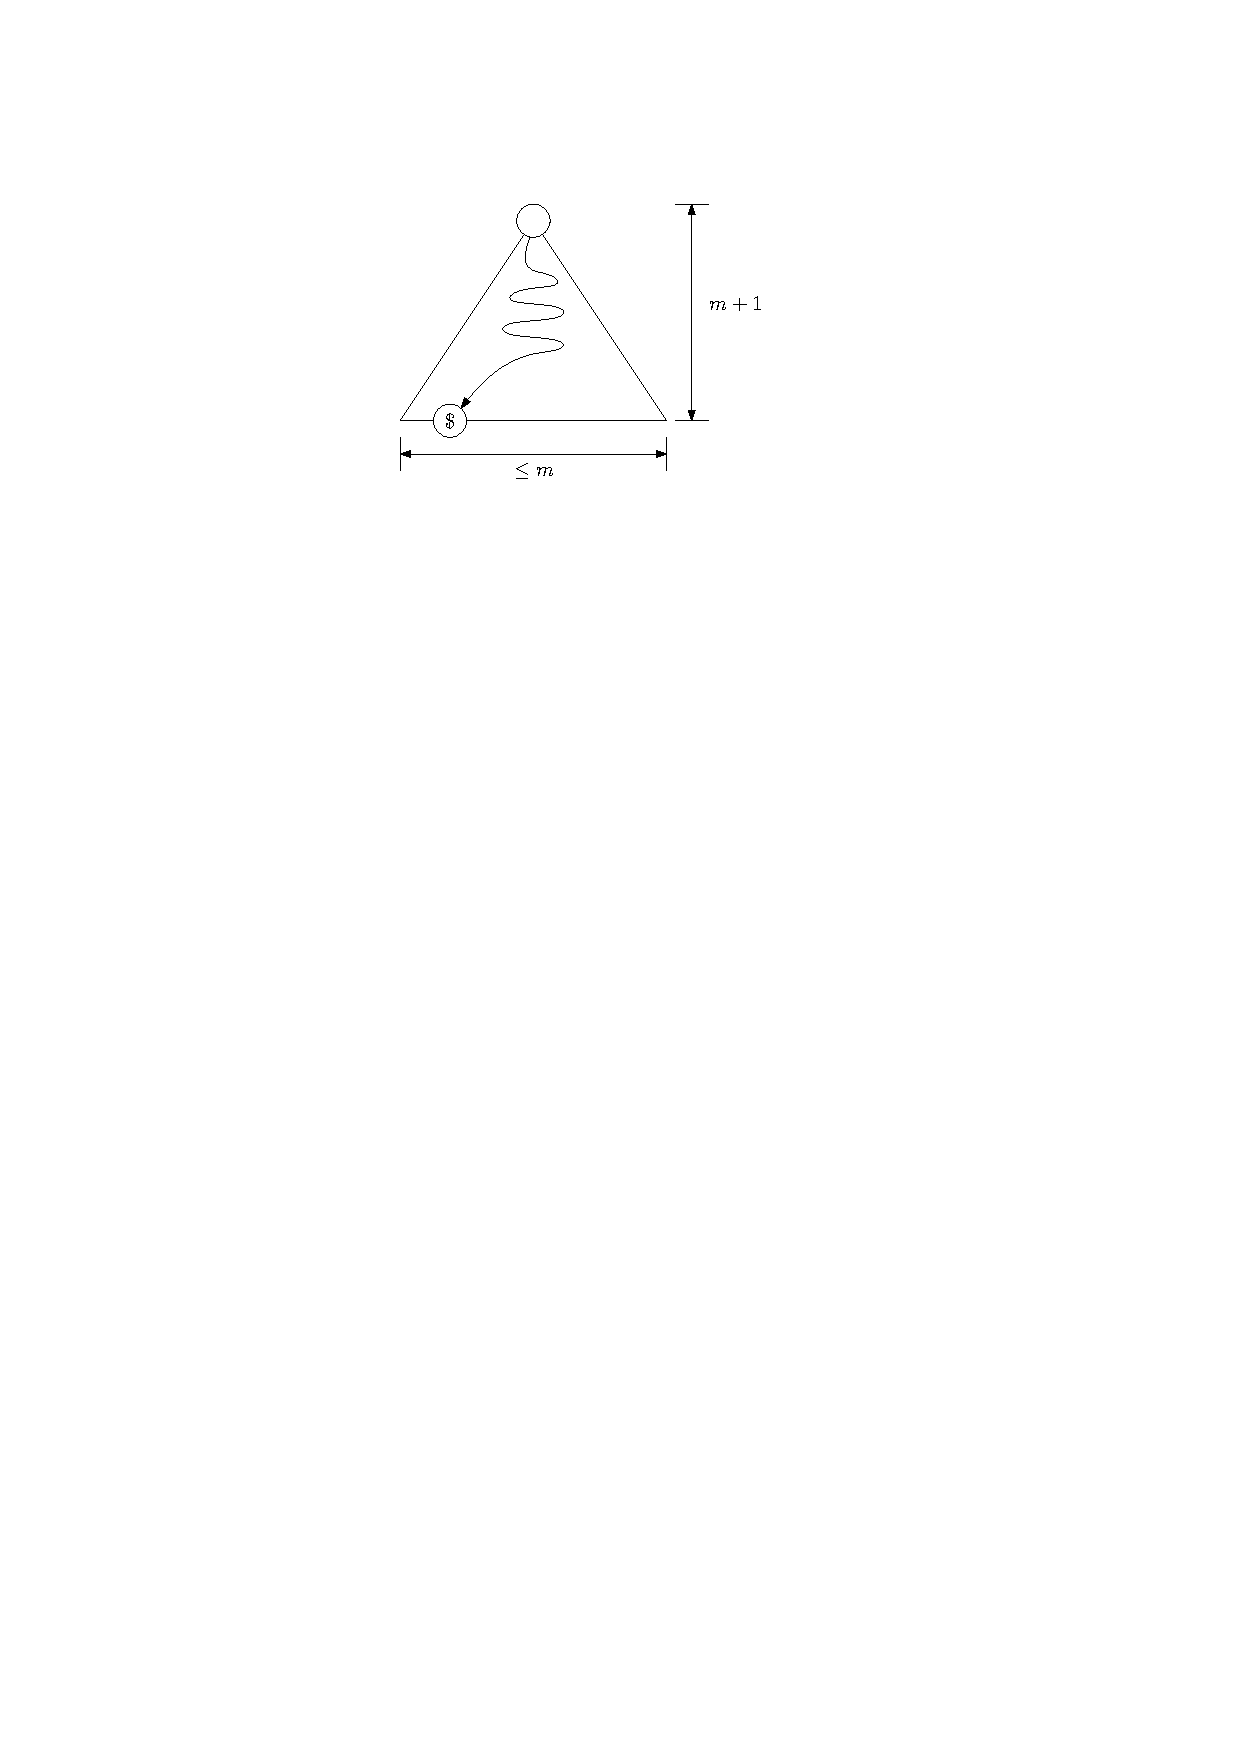
\includegraphics[width=\linewidth]{suffix-tree/suffix-trie-size.pdf}
    \caption{Max width and height of a suffix trie. The path from the root to the deepest leaf represents the longest suffix (the whole string plus the terminator).}
\end{marginfigure}

\subsection{Construct a Suffix Trie}

\section{Suffix Tree}

\subsection{From Suffix Trie to Suffix Tree}
